\documentclass{standalone}


\usepackage{pgfplots}

\begin{document}

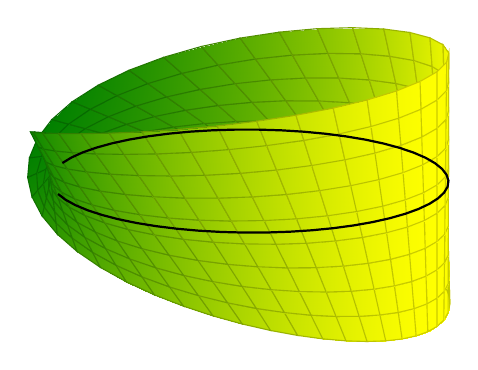
\begin{tikzpicture}
\begin{axis}[
    hide axis,
    view={20}{20}
]
\addplot3 [
    surf, shader=faceted interp,
    point meta=x,
    colormap/greenyellow,
    samples=40,
    samples y=10,
    z buffer=sort,
    domain=0:360,
    y domain=-0.5:0.5
] (
    {cos(x) -y*sin(x)*sin(x/2)},
    {sin(x) + y*cos(x)*sin(x/2)},
    {y*cos(x/2)});

\addplot3 [
    samples=50,
    domain=-145:180, % The domain needs to be adjusted manually, depending on the camera angle, unfortunately
    samples y=0,
    thick
] (
    {cos(x)},
    {sin(x)},
    {0});
\end{axis}
\end{tikzpicture}

\end{document}